% Created by tikzDevice version 0.12.3.1 on 2022-09-02 10:35:43
% !TEX encoding = UTF-8 Unicode
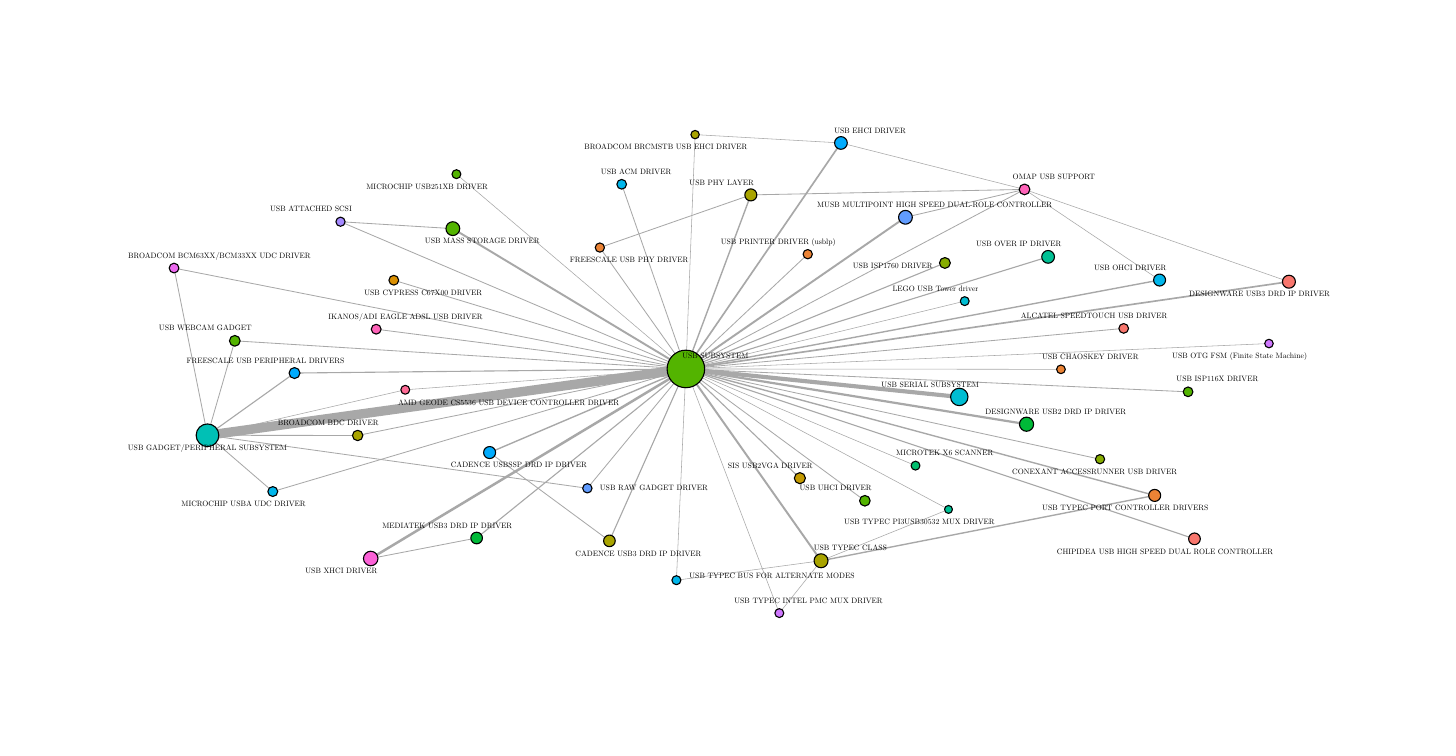
\begin{tikzpicture}[x=1pt,y=1pt]
\definecolor{fillColor}{RGB}{255,255,255}
\path[use as bounding box,fill=fillColor,fill opacity=0.00] (0,0) rectangle (505.89,252.94);
\begin{scope}
\path[clip] (  0.00,  0.00) rectangle (505.89,252.94);
\definecolor{fillColor}{RGB}{255,255,255}

\path[fill=fillColor] (  0.00,  0.00) rectangle (505.89,252.94);
\end{scope}
\begin{scope}
\path[clip] ( 32.75, 32.75) rectangle (475.89,222.94);
\definecolor{drawColor}{gray}{0.66}

\path[draw=drawColor,line width= 0.3pt,line join=round] (396.04,144.27) -- (237.84,129.62);

\path[draw=drawColor,line width= 0.2pt,line join=round] (136.44,122.09) -- ( 64.98,105.65);

\path[draw=drawColor,line width= 0.2pt,line join=round] (136.44,122.09) -- (237.84,129.62);

\path[draw=drawColor,line width= 0.3pt,line join=round] ( 52.89,166.07) -- ( 64.98,105.65);

\path[draw=drawColor,line width= 0.3pt,line join=round] ( 52.89,166.07) -- (237.84,129.62);

\path[draw=drawColor,line width= 0.3pt,line join=round] (119.24,105.58) -- ( 64.98,105.65);

\path[draw=drawColor,line width= 0.3pt,line join=round] (119.24,105.58) -- (237.84,129.62);

\path[draw=drawColor,line width= 0.2pt,line join=round] (241.17,214.30) -- (293.87,211.28);

\path[draw=drawColor,line width= 0.2pt,line join=round] (241.17,214.30) -- (237.84,129.62);

\path[draw=drawColor,line width= 0.3pt,line join=round] (210.21, 67.50) -- (166.92, 99.41);

\path[draw=drawColor,line width= 0.4pt,line join=round] (210.21, 67.50) -- (237.84,129.62);

\path[draw=drawColor,line width= 0.5pt,line join=round] (166.92, 99.41) -- (237.84,129.62);

\path[draw=drawColor,line width= 0.4pt,line join=round] (421.62, 68.23) -- (237.84,129.62);

\path[draw=drawColor,line width= 0.3pt,line join=round] (387.49, 97.01) -- (237.84,129.62);

\path[draw=drawColor,line width= 0.8pt,line join=round] (360.94,109.65) -- (237.84,129.62);

\path[draw=drawColor,line width= 0.2pt,line join=round] (455.75,161.14) -- (360.21,194.49);

\path[draw=drawColor,line width= 0.6pt,line join=round] (455.75,161.14) -- (237.84,129.62);

\path[draw=drawColor,line width= 0.4pt,line join=round] ( 96.42,128.14) -- ( 64.98,105.65);

\path[draw=drawColor,line width= 0.4pt,line join=round] ( 96.42,128.14) -- (237.84,129.62);

\path[draw=drawColor,line width= 0.3pt,line join=round] (206.75,173.48) -- (261.31,192.51);

\path[draw=drawColor,line width= 0.3pt,line join=round] (206.75,173.48) -- (237.84,129.62);

\path[draw=drawColor,line width= 0.3pt,line join=round] (125.93,143.98) -- (237.84,129.62);

\path[draw=drawColor,line width= 0.2pt,line join=round] (338.60,154.12) -- (237.84,129.62);

\path[draw=drawColor,line width= 0.4pt,line join=round] (162.23, 68.53) -- (237.84,129.62);

\path[draw=drawColor,line width= 0.3pt,line join=round] (162.23, 68.53) -- (123.96, 61.12);

\path[draw=drawColor,line width= 0.2pt,line join=round] (154.93,200.00) -- (237.84,129.62);

\path[draw=drawColor,line width= 0.3pt,line join=round] ( 88.57, 85.32) -- ( 64.98,105.65);

\path[draw=drawColor,line width= 0.3pt,line join=round] ( 88.57, 85.32) -- (237.84,129.62);

\path[draw=drawColor,line width= 0.2pt,line join=round] (320.82, 94.68) -- (237.84,129.62);

\path[draw=drawColor,line width= 0.3pt,line join=round] (317.18,184.42) -- (360.21,194.49);

\path[draw=drawColor,line width= 0.7pt,line join=round] (317.18,184.42) -- (237.84,129.62);

\path[draw=drawColor,line width= 0.2pt,line join=round] (360.21,194.49) -- (293.87,211.28);

\path[draw=drawColor,line width= 0.2pt,line join=round] (360.21,194.49) -- (409.01,161.74);

\path[draw=drawColor,line width= 0.3pt,line join=round] (360.21,194.49) -- (261.31,192.51);

\path[draw=drawColor,line width= 0.3pt,line join=round] (360.21,194.49) -- (237.84,129.62);

\path[draw=drawColor,line width= 0.4pt,line join=round] (279.03, 90.15) -- (237.84,129.62);

\path[draw=drawColor,line width= 0.3pt,line join=round] (214.64,196.35) -- (237.84,129.62);

\path[draw=drawColor,line width= 0.3pt,line join=round] (113.04,182.82) -- (153.63,180.32);

\path[draw=drawColor,line width= 0.3pt,line join=round] (113.04,182.82) -- (237.84,129.62);

\path[draw=drawColor,line width= 0.2pt,line join=round] (373.37,129.48) -- (237.84,129.62);

\path[draw=drawColor,line width= 0.3pt,line join=round] (132.30,161.68) -- (237.84,129.62);

\path[draw=drawColor,line width= 0.6pt,line join=round] (293.87,211.28) -- (237.84,129.62);

\path[draw=drawColor,line width= 0.3pt,line join=round] ( 64.98,105.65) -- (202.24, 86.50);

\path[draw=drawColor,line width= 3.4pt,line join=round] ( 64.98,105.65) -- (237.84,129.62);

\path[draw=drawColor,line width= 0.3pt,line join=round] ( 64.98,105.65) -- ( 74.85,139.78);

\path[draw=drawColor,line width= 0.3pt,line join=round] (419.31,121.35) -- (237.84,129.62);

\path[draw=drawColor,line width= 0.4pt,line join=round] (331.44,167.92) -- (237.84,129.62);

\path[draw=drawColor,line width= 0.7pt,line join=round] (153.63,180.32) -- (237.84,129.62);

\path[draw=drawColor,line width= 0.5pt,line join=round] (409.01,161.74) -- (237.84,129.62);

\path[draw=drawColor,line width= 0.2pt,line join=round] (448.54,138.80) -- (237.84,129.62);

\path[draw=drawColor,line width= 0.4pt,line join=round] (368.73,170.12) -- (237.84,129.62);

\path[draw=drawColor,line width= 0.5pt,line join=round] (261.31,192.51) -- (237.84,129.62);

\path[draw=drawColor,line width= 0.3pt,line join=round] (281.87,171.09) -- (237.84,129.62);

\path[draw=drawColor,line width= 0.3pt,line join=round] (202.24, 86.50) -- (237.84,129.62);

\path[draw=drawColor,line width= 1.5pt,line join=round] (336.64,119.50) -- (237.84,129.62);

\path[draw=drawColor,line width= 0.2pt,line join=round] (237.84,129.62) -- (234.42, 53.28);

\path[draw=drawColor,line width= 0.7pt,line join=round] (237.84,129.62) -- (286.68, 60.31);

\path[draw=drawColor,line width= 0.2pt,line join=round] (237.84,129.62) -- (271.60, 41.40);

\path[draw=drawColor,line width= 0.2pt,line join=round] (237.84,129.62) -- (332.74, 78.86);

\path[draw=drawColor,line width= 0.5pt,line join=round] (237.84,129.62) -- (407.24, 83.92);

\path[draw=drawColor,line width= 0.3pt,line join=round] (237.84,129.62) -- (302.52, 81.99);

\path[draw=drawColor,line width= 0.3pt,line join=round] (237.84,129.62) -- ( 74.85,139.78);

\path[draw=drawColor,line width= 0.9pt,line join=round] (237.84,129.62) -- (123.96, 61.12);

\path[draw=drawColor,line width= 0.2pt,line join=round] (234.42, 53.28) -- (286.68, 60.31);

\path[draw=drawColor,line width= 0.2pt,line join=round] (286.68, 60.31) -- (271.60, 41.40);

\path[draw=drawColor,line width= 0.2pt,line join=round] (286.68, 60.31) -- (332.74, 78.86);

\path[draw=drawColor,line width= 0.5pt,line join=round] (286.68, 60.31) -- (407.24, 83.92);
\definecolor{drawColor}{RGB}{0,0,0}
\definecolor{fillColor}{RGB}{248,118,109}

\path[draw=drawColor,line width= 0.4pt,line join=round,line cap=round,fill=fillColor] (396.04,144.27) circle (  1.75);
\definecolor{fillColor}{RGB}{255,107,150}

\path[draw=drawColor,line width= 0.4pt,line join=round,line cap=round,fill=fillColor] (136.44,122.09) circle (  1.61);
\definecolor{fillColor}{RGB}{236,105,239}

\path[draw=drawColor,line width= 0.4pt,line join=round,line cap=round,fill=fillColor] ( 52.89,166.07) circle (  1.76);
\definecolor{fillColor}{RGB}{169,164,0}

\path[draw=drawColor,line width= 0.4pt,line join=round,line cap=round,fill=fillColor] (119.24,105.58) circle (  1.88);

\path[draw=drawColor,line width= 0.4pt,line join=round,line cap=round,fill=fillColor] (241.17,214.30) circle (  1.51);

\path[draw=drawColor,line width= 0.4pt,line join=round,line cap=round,fill=fillColor] (210.21, 67.50) circle (  2.10);
\definecolor{fillColor}{RGB}{0,171,253}

\path[draw=drawColor,line width= 0.4pt,line join=round,line cap=round,fill=fillColor] (166.92, 99.41) circle (  2.17);
\definecolor{fillColor}{RGB}{248,118,109}

\path[draw=drawColor,line width= 0.4pt,line join=round,line cap=round,fill=fillColor] (421.62, 68.23) circle (  2.11);
\definecolor{fillColor}{RGB}{134,172,0}

\path[draw=drawColor,line width= 0.4pt,line join=round,line cap=round,fill=fillColor] (387.49, 97.01) circle (  1.67);
\definecolor{fillColor}{RGB}{0,186,56}

\path[draw=drawColor,line width= 0.4pt,line join=round,line cap=round,fill=fillColor] (360.94,109.65) circle (  2.55);
\definecolor{fillColor}{RGB}{248,118,109}

\path[draw=drawColor,line width= 0.4pt,line join=round,line cap=round,fill=fillColor] (455.75,161.14) circle (  2.34);
\definecolor{fillColor}{RGB}{0,171,253}

\path[draw=drawColor,line width= 0.4pt,line join=round,line cap=round,fill=fillColor] ( 96.42,128.14) circle (  1.98);
\definecolor{fillColor}{RGB}{235,131,53}

\path[draw=drawColor,line width= 0.4pt,line join=round,line cap=round,fill=fillColor] (206.75,173.48) circle (  1.67);
\definecolor{fillColor}{RGB}{255,99,185}

\path[draw=drawColor,line width= 0.4pt,line join=round,line cap=round,fill=fillColor] (125.93,143.98) circle (  1.78);
\definecolor{fillColor}{RGB}{0,189,210}

\path[draw=drawColor,line width= 0.4pt,line join=round,line cap=round,fill=fillColor] (338.60,154.12) circle (  1.61);
\definecolor{fillColor}{RGB}{0,186,56}

\path[draw=drawColor,line width= 0.4pt,line join=round,line cap=round,fill=fillColor] (162.23, 68.53) circle (  2.10);
\definecolor{fillColor}{RGB}{83,180,0}

\path[draw=drawColor,line width= 0.4pt,line join=round,line cap=round,fill=fillColor] (154.93,200.00) circle (  1.61);
\definecolor{fillColor}{RGB}{0,182,235}

\path[draw=drawColor,line width= 0.4pt,line join=round,line cap=round,fill=fillColor] ( 88.57, 85.32) circle (  1.79);
\definecolor{fillColor}{RGB}{0,190,109}

\path[draw=drawColor,line width= 0.4pt,line join=round,line cap=round,fill=fillColor] (320.82, 94.68) circle (  1.61);
\definecolor{fillColor}{RGB}{97,156,255}

\path[draw=drawColor,line width= 0.4pt,line join=round,line cap=round,fill=fillColor] (317.18,184.42) circle (  2.49);
\definecolor{fillColor}{RGB}{255,99,185}

\path[draw=drawColor,line width= 0.4pt,line join=round,line cap=round,fill=fillColor] (360.21,194.49) circle (  1.94);
\definecolor{fillColor}{RGB}{196,154,0}

\path[draw=drawColor,line width= 0.4pt,line join=round,line cap=round,fill=fillColor] (279.03, 90.15) circle (  2.01);
\definecolor{fillColor}{RGB}{0,182,235}

\path[draw=drawColor,line width= 0.4pt,line join=round,line cap=round,fill=fillColor] (214.64,196.35) circle (  1.75);
\definecolor{fillColor}{RGB}{165,138,255}

\path[draw=drawColor,line width= 0.4pt,line join=round,line cap=round,fill=fillColor] (113.04,182.82) circle (  1.66);
\definecolor{fillColor}{RGB}{235,131,53}

\path[draw=drawColor,line width= 0.4pt,line join=round,line cap=round,fill=fillColor] (373.37,129.48) circle (  1.57);
\definecolor{fillColor}{RGB}{218,143,0}

\path[draw=drawColor,line width= 0.4pt,line join=round,line cap=round,fill=fillColor] (132.30,161.68) circle (  1.77);
\definecolor{fillColor}{RGB}{0,171,253}

\path[draw=drawColor,line width= 0.4pt,line join=round,line cap=round,fill=fillColor] (293.87,211.28) circle (  2.29);
\definecolor{fillColor}{RGB}{0,192,181}

\path[draw=drawColor,line width= 0.4pt,line join=round,line cap=round,fill=fillColor] ( 64.98,105.65) circle (  4.10);
\definecolor{fillColor}{RGB}{83,180,0}

\path[draw=drawColor,line width= 0.4pt,line join=round,line cap=round,fill=fillColor] (419.31,121.35) circle (  1.75);
\definecolor{fillColor}{RGB}{134,172,0}

\path[draw=drawColor,line width= 0.4pt,line join=round,line cap=round,fill=fillColor] (331.44,167.92) circle (  1.96);
\definecolor{fillColor}{RGB}{83,180,0}

\path[draw=drawColor,line width= 0.4pt,line join=round,line cap=round,fill=fillColor] (153.63,180.32) circle (  2.49);
\definecolor{fillColor}{RGB}{0,182,235}

\path[draw=drawColor,line width= 0.4pt,line join=round,line cap=round,fill=fillColor] (409.01,161.74) circle (  2.16);
\definecolor{fillColor}{RGB}{208,120,255}

\path[draw=drawColor,line width= 0.4pt,line join=round,line cap=round,fill=fillColor] (448.54,138.80) circle (  1.54);
\definecolor{fillColor}{RGB}{0,192,148}

\path[draw=drawColor,line width= 0.4pt,line join=round,line cap=round,fill=fillColor] (368.73,170.12) circle (  2.30);
\definecolor{fillColor}{RGB}{169,164,0}

\path[draw=drawColor,line width= 0.4pt,line join=round,line cap=round,fill=fillColor] (261.31,192.51) circle (  2.17);
\definecolor{fillColor}{RGB}{235,131,53}

\path[draw=drawColor,line width= 0.4pt,line join=round,line cap=round,fill=fillColor] (281.87,171.09) circle (  1.68);
\definecolor{fillColor}{RGB}{97,156,255}

\path[draw=drawColor,line width= 0.4pt,line join=round,line cap=round,fill=fillColor] (202.24, 86.50) circle (  1.69);
\definecolor{fillColor}{RGB}{0,189,210}

\path[draw=drawColor,line width= 0.4pt,line join=round,line cap=round,fill=fillColor] (336.64,119.50) circle (  3.14);
\definecolor{fillColor}{RGB}{83,180,0}

\path[draw=drawColor,line width= 0.4pt,line join=round,line cap=round,fill=fillColor] (237.84,129.62) circle (  6.78);
\definecolor{fillColor}{RGB}{0,182,235}

\path[draw=drawColor,line width= 0.4pt,line join=round,line cap=round,fill=fillColor] (234.42, 53.28) circle (  1.63);
\definecolor{fillColor}{RGB}{169,164,0}

\path[draw=drawColor,line width= 0.4pt,line join=round,line cap=round,fill=fillColor] (286.68, 60.31) circle (  2.52);
\definecolor{fillColor}{RGB}{208,120,255}

\path[draw=drawColor,line width= 0.4pt,line join=round,line cap=round,fill=fillColor] (271.60, 41.40) circle (  1.61);
\definecolor{fillColor}{RGB}{0,192,148}

\path[draw=drawColor,line width= 0.4pt,line join=round,line cap=round,fill=fillColor] (332.74, 78.86) circle (  1.43);
\definecolor{fillColor}{RGB}{235,131,53}

\path[draw=drawColor,line width= 0.4pt,line join=round,line cap=round,fill=fillColor] (407.24, 83.92) circle (  2.17);
\definecolor{fillColor}{RGB}{83,180,0}

\path[draw=drawColor,line width= 0.4pt,line join=round,line cap=round,fill=fillColor] (302.52, 81.99) circle (  1.92);

\path[draw=drawColor,line width= 0.4pt,line join=round,line cap=round,fill=fillColor] ( 74.85,139.78) circle (  1.94);
\definecolor{fillColor}{RGB}{251,97,215}

\path[draw=drawColor,line width= 0.4pt,line join=round,line cap=round,fill=fillColor] (123.96, 61.12) circle (  2.62);

\node[text=drawColor,anchor=base,inner sep=0pt, outer sep=0pt, scale=  0.28] at (385.37,147.88) {ALCATEL SPEEDTOUCH USB DRIVER};

\node[text=drawColor,anchor=base,inner sep=0pt, outer sep=0pt, scale=  0.28] at (173.75,116.59) {AMD GEODE CS5536 USB DEVICE CONTROLLER DRIVER};

\node[text=drawColor,anchor=base,inner sep=0pt, outer sep=0pt, scale=  0.28] at ( 69.28,169.61) {BROADCOM BCM63XX/BCM33XX UDC DRIVER};

\node[text=drawColor,anchor=base,inner sep=0pt, outer sep=0pt, scale=  0.28] at (108.60,109.20) {BROADCOM BDC DRIVER};

\node[text=drawColor,anchor=base,inner sep=0pt, outer sep=0pt, scale=  0.28] at (230.62,208.78) {BROADCOM BRCMSTB USB EHCI DRIVER};

\node[text=drawColor,anchor=base,inner sep=0pt, outer sep=0pt, scale=  0.28] at (220.68, 62.01) {CADENCE USB3 DRD IP DRIVER};

\node[text=drawColor,anchor=base,inner sep=0pt, outer sep=0pt, scale=  0.28] at (177.49, 93.91) {CADENCE USBSSP DRD IP DRIVER};

\node[text=drawColor,anchor=base,inner sep=0pt, outer sep=0pt, scale=  0.28] at (410.98, 62.65) {CHIPIDEA USB HIGH SPEED DUAL ROLE CONTROLLER};

\node[text=drawColor,anchor=base,inner sep=0pt, outer sep=0pt, scale=  0.28] at (385.56, 91.46) {CONEXANT ACCESSRUNNER USB DRIVER};

\node[text=drawColor,anchor=base,inner sep=0pt, outer sep=0pt, scale=  0.28] at (371.50,113.18) {DESIGNWARE USB2 DRD IP DRIVER};

\node[text=drawColor,anchor=base,inner sep=0pt, outer sep=0pt, scale=  0.28] at (445.14,155.63) {DESIGNWARE USB3 DRD IP DRIVER};

\node[text=drawColor,anchor=base,inner sep=0pt, outer sep=0pt, scale=  0.28] at ( 85.91,131.68) {FREESCALE USB PERIPHERAL DRIVERS};

\node[text=drawColor,anchor=base,inner sep=0pt, outer sep=0pt, scale=  0.28] at (217.34,167.94) {FREESCALE USB PHY DRIVER};

\node[text=drawColor,anchor=base,inner sep=0pt, outer sep=0pt, scale=  0.28] at (136.49,147.55) {IKANOS/ADI EAGLE ADSL USB DRIVER};

\node[text=drawColor,anchor=base,inner sep=0pt, outer sep=0pt, scale=  0.28] at (328.06,157.67) {LEGO USB Tower driver};

\node[text=drawColor,anchor=base,inner sep=0pt, outer sep=0pt, scale=  0.28] at (151.61, 72.11) {MEDIATEK USB3 DRD IP DRIVER};

\node[text=drawColor,anchor=base,inner sep=0pt, outer sep=0pt, scale=  0.28] at (144.32,194.46) {MICROCHIP USB251XB DRIVER};

\node[text=drawColor,anchor=base,inner sep=0pt, outer sep=0pt, scale=  0.28] at ( 77.99, 79.78) {MICROCHIP USBA UDC DRIVER};

\node[text=drawColor,anchor=base,inner sep=0pt, outer sep=0pt, scale=  0.28] at (331.38, 98.25) {MICROTEK X6 SCANNER};

\node[text=drawColor,anchor=base,inner sep=0pt, outer sep=0pt, scale=  0.28] at (327.72,187.98) {MUSB MULTIPOINT HIGH SPEED DUAL-ROLE CONTROLLER};

\node[text=drawColor,anchor=base,inner sep=0pt, outer sep=0pt, scale=  0.28] at (370.83,198.06) {OMAP USB SUPPORT};

\node[text=drawColor,anchor=base,inner sep=0pt, outer sep=0pt, scale=  0.28] at (268.34, 93.73) {SIS USB2VGA DRIVER};

\node[text=drawColor,anchor=base,inner sep=0pt, outer sep=0pt, scale=  0.28] at (219.86,199.91) {USB ACM DRIVER};

\node[text=drawColor,anchor=base,inner sep=0pt, outer sep=0pt, scale=  0.28] at (102.38,186.44) {USB ATTACHED SCSI};

\node[text=drawColor,anchor=base,inner sep=0pt, outer sep=0pt, scale=  0.28] at (383.96,133.07) {USB CHAOSKEY DRIVER};

\node[text=drawColor,anchor=base,inner sep=0pt, outer sep=0pt, scale=  0.28] at (142.92,156.16) {USB CYPRESS C67X00 DRIVER};

\node[text=drawColor,anchor=base,inner sep=0pt, outer sep=0pt, scale=  0.28] at (304.37,214.82) {USB EHCI DRIVER};

\node[text=drawColor,anchor=base,inner sep=0pt, outer sep=0pt, scale=  0.28] at ( 64.97,100.13) {USB GADGET/PERIPHERAL SUBSYSTEM};

\node[text=drawColor,anchor=base,inner sep=0pt, outer sep=0pt, scale=  0.28] at (429.90,124.91) {USB ISP116X DRIVER};

\node[text=drawColor,anchor=base,inner sep=0pt, outer sep=0pt, scale=  0.28] at (312.58,165.76) {USB ISP1760 DRIVER};

\node[text=drawColor,anchor=base,inner sep=0pt, outer sep=0pt, scale=  0.28] at (164.27,174.79) {USB MASS STORAGE DRIVER};

\node[text=drawColor,anchor=base,inner sep=0pt, outer sep=0pt, scale=  0.28] at (398.42,165.29) {USB OHCI DRIVER};

\node[text=drawColor,anchor=base,inner sep=0pt, outer sep=0pt, scale=  0.28] at (437.96,133.30) {USB OTG FSM (Finite State Machine)};

\node[text=drawColor,anchor=base,inner sep=0pt, outer sep=0pt, scale=  0.28] at (358.14,173.71) {USB OVER IP DRIVER};

\node[text=drawColor,anchor=base,inner sep=0pt, outer sep=0pt, scale=  0.28] at (250.78,196.07) {USB PHY LAYER};

\node[text=drawColor,anchor=base,inner sep=0pt, outer sep=0pt, scale=  0.28] at (271.23,174.68) {USB PRINTER DRIVER (usblp)};

\node[text=drawColor,anchor=base,inner sep=0pt, outer sep=0pt, scale=  0.28] at (226.28, 85.85) {USB RAW GADGET DRIVER};

\node[text=drawColor,anchor=base,inner sep=0pt, outer sep=0pt, scale=  0.28] at (326.13,123.06) {USB SERIAL SUBSYSTEM};

\node[text=drawColor,anchor=base,inner sep=0pt, outer sep=0pt, scale=  0.28] at (248.49,133.23) {USB SUBSYSTEM};

\node[text=drawColor,anchor=base,inner sep=0pt, outer sep=0pt, scale=  0.28] at (268.99, 53.96) {USB TYPEC BUS FOR ALTERNATE MODES};

\node[text=drawColor,anchor=base,inner sep=0pt, outer sep=0pt, scale=  0.28] at (297.28, 63.87) {USB TYPEC CLASS};

\node[text=drawColor,anchor=base,inner sep=0pt, outer sep=0pt, scale=  0.28] at (282.15, 44.96) {USB TYPEC INTEL PMC MUX DRIVER};

\node[text=drawColor,anchor=base,inner sep=0pt, outer sep=0pt, scale=  0.28] at (322.22, 73.33) {USB TYPEC PI3USB30532 MUX DRIVER};

\node[text=drawColor,anchor=base,inner sep=0pt, outer sep=0pt, scale=  0.28] at (396.63, 78.39) {USB TYPEC PORT CONTROLLER DRIVERS};

\node[text=drawColor,anchor=base,inner sep=0pt, outer sep=0pt, scale=  0.28] at (291.96, 85.52) {USB UHCI DRIVER};

\node[text=drawColor,anchor=base,inner sep=0pt, outer sep=0pt, scale=  0.28] at ( 64.20,143.40) {USB WEBCAM GADGET};

\node[text=drawColor,anchor=base,inner sep=0pt, outer sep=0pt, scale=  0.28] at (113.36, 55.61) {USB XHCI DRIVER};
\end{scope}
\end{tikzpicture}
